%%%%%%%%%%%%%%%%%%%%%%%%%%%%%%%%%%%%%%%%%%%%%%%%%%%%%%%%%%%%%%%%%%%%%%
%%  Copyright by Wenliang Du.                                       %%
%%  This work is licensed under the Creative Commons                %%
%%  Attribution-NonCommercial-ShareAlike 4.0 International License. %%
%%  To view a copy of this license, visit                           %%
%%  http://creativecommons.org/licenses/by-nc-sa/4.0/.              %%
%%%%%%%%%%%%%%%%%%%%%%%%%%%%%%%%%%%%%%%%%%%%%%%%%%%%%%%%%%%%%%%%%%%%%%


\newcommand{\commonfolder}{../../common-files}

\documentclass[11pt]{article}

\usepackage[most]{tcolorbox}
\usepackage{times}
\usepackage{epsf}
\usepackage{epsfig}
\usepackage{amsmath, alltt, amssymb, xspace}
\usepackage{wrapfig}
\usepackage{fancyhdr}
\usepackage{url}
\usepackage{verbatim}
\usepackage{fancyvrb}
\usepackage{adjustbox}
\usepackage{listings}
\usepackage{color}
\usepackage{subfigure}
\usepackage{cite}
\usepackage{sidecap}
\usepackage{pifont}
\usepackage{mdframed}
\usepackage{textcomp}
\usepackage{enumitem}


% Horizontal alignment
\topmargin      -0.50in  % distance to headers
\oddsidemargin  0.0in
\evensidemargin 0.0in
\textwidth      6.5in
\textheight     8.9in 

\newcommand{\todo}[1]{
\vspace{0.1in}
\fbox{\parbox{6in}{TODO: #1}}
\vspace{0.1in}
}


\newcommand{\unix}{{\tt Unix}\xspace}
\newcommand{\linux}{{\tt Linux}\xspace}
\newcommand{\minix}{{\tt Minix}\xspace}
\newcommand{\ubuntu}{{\tt Ubuntu}\xspace}
\newcommand{\setuid}{{\tt Set-UID}\xspace}
\newcommand{\openssl} {\texttt{openssl}}


\pagestyle{fancy}
\lhead{\bfseries SEED Labs}
\chead{}
\rhead{\small \thepage}
\lfoot{}
\cfoot{}
\rfoot{}


\definecolor{dkgreen}{rgb}{0,0.6,0}
\definecolor{gray}{rgb}{0.5,0.5,0.5}
\definecolor{mauve}{rgb}{0.58,0,0.82}
\definecolor{lightgray}{gray}{0.90}


\lstset{%
  frame=none,
  language=,
  backgroundcolor=\color{lightgray},
  aboveskip=3mm,
  belowskip=3mm,
  showstringspaces=false,
%  columns=flexible,
  basicstyle={\small\ttfamily},
  numbers=none,
  numberstyle=\tiny\color{gray},
  keywordstyle=\color{blue},
  commentstyle=\color{dkgreen},
  stringstyle=\color{mauve},
  breaklines=true,
  breakatwhitespace=true,
  tabsize=3,
  columns=fullflexible,
  keepspaces=true,
  escapeinside={(*@}{@*)}
}

\newcommand{\newnote}[1]{
\vspace{0.1in}
\noindent
\fbox{\parbox{1.0\textwidth}{\textbf{Note:} #1}}
%\vspace{0.1in}
}


%% Submission
\newcommand{\seedsubmission}{You need to submit a detailed lab report, with screenshots,
to describe what you have done and what you have observed.
You also need to provide explanation
to the observations that are interesting or surprising.
Please also list the important code snippets followed by
explanation. Simply attaching code without any explanation will not
receive credits.}

%% Book
\newcommand{\seedbook}{\textit{Computer \& Internet Security: A Hands-on Approach}, 2nd
Edition, by Wenliang Du. See details at \url{https://www.handsonsecurity.net}.}

%% Videos
\newcommand{\seedisvideo}{\textit{Internet Security: A Hands-on Approach},
by Wenliang Du. See details at \url{https://www.handsonsecurity.net/video.html}.}

\newcommand{\seedcsvideo}{\textit{Computer Security: A Hands-on Approach},
by Wenliang Du. See details at \url{https://www.handsonsecurity.net/video.html}.}

%% Lab Environment
\newcommand{\seedenvironment}{This lab has been tested on our pre-built
Ubuntu 16.04 VM, which can be downloaded from the SEED website. }

\newcommand{\seedenvironmentA}{This lab has been tested on our pre-built
Ubuntu 16.04 VM, which can be downloaded from the SEED website. }

\newcommand{\seedenvironmentB}{This lab has been tested on our pre-built
Ubuntu 20.04 VM, which can be downloaded from the SEED website. }

\newcommand{\seedenvironmentAB}{This lab has been tested on our pre-built
Ubuntu 16.04 and 20.04 VMs, which can be downloaded from the SEED website. }

\newcommand{\nodependency}{Since we use containers to set up the lab environment, 
this lab does not depend too much on our SEED VM. You can do this lab
using other VMs or physical machines. }







\newcommand{\seedlabcopyright}[1]{
\vspace{0.1in}
\fbox{\parbox{6in}{\small Copyright \copyright\ {#1}\ \ by Wenliang Du.\\
      This work is licensed under a Creative Commons
      Attribution-NonCommercial-ShareAlike 4.0 International License.
      If you remix, transform, or build upon the material, 
      this copyright notice must be left intact, or reproduced in a way that is reasonable to
      the medium in which the work is being re-published.}}
\vspace{0.1in}
}






\newcommand{\tlsFigs}{./Figs}


\newcommand{\hostu}{{\tt U}\xspace}
\newcommand{\hostv}{{\tt V}\xspace}


\begin{document}

\begin{center}
{\LARGE Transport Layer Security (TLS) Lab}
\end{center}

\seedlabcopyright{2020}



% *******************************************
% SECTION
% *******************************************
\section{Overview}

Nowadays more and more data transmissions are done through the Internet. However, when data are
transmitted over such a public network unprotected, they can be
read or even modified by others. Applications worrying
about the security of their communication need to encrypt their data and
detect tampering. Cryptographic solutions can be used to achieve this goal.
There are many cryptographic algorithms, and even for the same
algorithm, there are many parameters that can be used. To achieve interoperability, i.e.,
allowing different applications to communicate with one another, these
applications need to follow a common standard. TLS, Transport Layer Security, is such a standard.
Most web servers these days are using HTTPS, which is built on top of TLS.

The objective of this lab is to help students understand how the TLS works and how 
to use TLS in programming. The lab
guides students to implement a pair of TLS client and server programs, based on
which students will conduct a series of experiments, so they can understand the 
security principles underlying the TLS protocol. Students will also
implement a simple HTTPS proxy program to understand the security 
impact if some trusted CAs are compromised. 
The lab covers the following topics:

\begin{itemize}[noitemsep]
\item Public-Key Infrastructure (PKI)
\item Transport Layer Security (TLS)
\item TLS programming
\item HTTPS proxy 
\item X.509 certificates with the Subject Alternative Name (SAN) extensions
\item Man-In-The-Middle attacks
\end{itemize}


\paragraph{Prerequisite.} This lab depends on the PKI lab. Students should 
do the PKI lab before working on this lab. 

\paragraph{Readings.}
Detailed coverage of PKI and TLS can be found in the following:

\begin{itemize}
\item Chapters 24 and 25 of the SEED Book, \seedbook
\end{itemize}


\paragraph{Lab Environment.} \seedenvironmentB


%Note: there are two SSL wrapper modules in Python, one is 
%ssl and the other is pyopenssl. We will mainly use ssl, which 
%seems more popular. 
%It should be noted that directly using C, you will have 
%more options, because not everything 
%in the openssl library has been implemented by the Python wrapper. 


\newpage

% *******************************************
% SECTION
% *******************************************
\section{Lab Environment}

In this lab, we use three machines, one for client, one for server,
and the other for proxy. We will use containers for these machines.  
Their IP addresses are listed in the following:


\begin{lstlisting}
client: 10.9.0.5
server: 10.9.0.43
proxy:  10.9.0.143
\end{lstlisting}
 


\paragraph{Container Setup and Commands.}
%%%%%%%%%%%%%%%%%%%%%%%%%%%%%%%%%%%%%%%%%%%%
Please download the
\texttt{Labsetup.zip} file to your VM from the lab's website,
unzip it, enter the \texttt{Labsetup} folder, and 
use the \texttt{docker-compose.yml} file to 
set up the lab environment. Detailed explanation
of the content in this file and all the involved 
\texttt{Dockerfile} can be found from the 
user manual, which is linked to the website of this lab.
If this is the first time you set up a SEED lab environment
using containers, it is very important that you read 
the user manual. 

In the following, we list some of the commonly
used commands related to Docker and Compose. 
Since we are going to use 
these commands very frequently, we have created aliases for them
in the \texttt{.bashrc} file (in our provided SEEDUbuntu 20.04 VM).


\begin{lstlisting}
$ docker-compose build  # Build the container image
$ docker-compose up     # Start the container
$ docker-compose down   # Shut down the container

// Aliases for the Compose commands above
$ dcbuild       # Alias for: docker-compose build
$ dcup          # Alias for: docker-compose up
$ dcdown        # Alias for: docker-compose down
\end{lstlisting}


All the containers will be running in the background. To run
commands on a container, we often need to get a shell on
that container. We first need to use the \texttt{"docker ps"}  
command to find out the ID of the container, and then
use \texttt{"docker exec"} to start a shell on that 
container. We have created aliases for them in
the \texttt{.bashrc} file.

\begin{lstlisting}
$ dockps        # Alias for: docker ps --format "{{.ID}}  {{.Names}}" 
$ docksh <id>   # Alias for: docker exec -it <id> /bin/bash

# The following example shows how to get a shell inside hostC
$ dockps
b1004832e275  hostA-10.9.0.5
0af4ea7a3e2e  hostB-10.9.0.6
9652715c8e0a  hostC-10.9.0.7

$ docksh 96
root@9652715c8e0a:/#  

# Note: If a docker command requires a container ID, you do not need to 
#       type the entire ID string. Typing the first few characters will 
#       be sufficient, as long as they are unique among all the containers. 
\end{lstlisting}


If you encounter problems when setting up the lab environment, 
please read the ``Common Problems'' section of the manual
for potential solutions.


%%%%%%%%%%%%%%%%%%%%%%%%%%%%%%%%%%%%%%%%%%%%



\paragraph{Volumes.} 
%%%%%%%%%%%%%%%%%%%%%%%%%%%%%%%%%%%%%%%%%%%%
Code editing is more convenient inside the VM than in a container, 
because we can use our favorite editor to write code. 
In order for the VM and a container to share files, 
we have created a shared folder between VM and the container
using the Docker \texttt{volumes}.
If you look at the Docker Compose file, you will find out that
we have added the following entry to some of the containers.
It indicates mounting the \texttt{./volumes} folder on the host
machine (i.e., the VM) to the \texttt{/volumes} folder inside the container.
We will write our code in the \texttt{./volumes} folder (on the VM), so they
can be used inside the containers.

\begin{lstlisting}
volumes:
       - ./volumes:/volumes
\end{lstlisting}


%%%%%%%%%%%%%%%%%%%%%%%%%%%%%%%%%%%%%%%%%%%%





% *******************************************
% SECTION
% ******************************************* 
\section{Task 1: TLS Client}


In this task, we will incrementally build a simple TLS 
client program. Through the process, students will 
understand the essential elements and 
security considerations in TLS programming. We will run 
this client program on the client container.


% -------------------------------------------
% SUBSECTION
% ------------------------------------------- 
\subsection{Task 1.a: TLS handshake}


Before a client and a server can communicate securely, several things need to be set up first,
including what encryption algorithm and key will be used, what MAC algorithm will be used, what
algorithm should be used for the key exchange, etc. These cryptographic parameters need to be
agreed upon by the client and the server. That is the primary purpose of the TLS Handshake
Protocol. In this task, we focus on the TLS handshake protocol. 
The following sample code initiates a TLS handshake with
a TLS server (the name of the server needs to be specified as the first command line argument).


\begin{lstlisting}[caption={\texttt{handshake.py}}, label={tls:handshake}]
#!/usr/bin/env python3

import socket, ssl, sys, pprint

hostname = sys.argv[1]
port = 443
cadir = '/etc/ssl/certs'   

# Set up the TLS context 
context = ssl.SSLContext(ssl.PROTOCOL_TLS_CLIENT) 
context.load_verify_locations(capath=cadir)
context.verify_mode = ssl.CERT_REQUIRED
context.check_hostname = True

# Create TCP connection 
sock = socket.socket(socket.AF_INET, socket.SOCK_STREAM)
sock.connect((hostname, port))
input("After making TCP connection. Press any key to continue ...")

# Add the TLS 
ssock = context.wrap_socket(sock, server_hostname=hostname,
                            do_handshake_on_connect=False)
ssock.do_handshake()   # Start the handshake
pprint.pprint(ssock.getpeercert())
input("After handshake. Press any key to continue ...")

# Close the TLS Connection
ssock.shutdown(socket.SHUT_RDWR)
ssock.close()
\end{lstlisting}
 
%print("=== Cipher used: {}".format(ssock.cipher()))
%print("=== Server hostname: {}".format(ssock.server_hostname))
%print("=== Server certificate:")



\paragraph{Tasks.} Use the code above to communicate with a real HTTPS-based web server.
Additional code may need to be added to complete the tasks. Students can find the manual
for Python's SSL module online.  Please report the following:
\begin{itemize}
\item What is the cipher used between the client and the server? 
\item Please print out the server certificate in the program.
\item Explain the purpose of \texttt{/etc/ssl/certs}.
\item Use Wireshark to capture the network traffics during the 
execution of the program, and explain your observation. In particular,
explain which step triggers the TCP handshake, and which
step triggers the TLS handshake. Explain the relationship between
 the TLS handshake and the TCP handshake. 
\end{itemize}
 


% -------------------------------------------
% SUBSECTION
% ------------------------------------------- 
\subsection{Task 1.b: CA's Certificate}

In the previous task, we use the certificates in
the \texttt{/etc/ssl/certs} folder to verify server's certificates. In this task,
we will create our own certificate folder, and place the corresponding 
certificates in the folder to do the verification.


Please create a folder called \texttt{certs}, and change the 
\texttt{cadir} line in the client program to the following. Run the client program
and report your observation.

\begin{lstlisting}
cadir = './certs'   
\end{lstlisting}


To solve this problem, you need to place the corresponding CA's certificate 
into your \texttt{certs} folder.  Please use your client program
to find out what CA certificate is needed to verify
the \texttt{www.example.com} server's certificate, and then copy
the certificate from the \texttt{/etc/ssl/certs} to your 
own folder. Run your client program again. If you have done everything correctly,
your client program should be able to talk to the server.


It should be noted that copying CA's certificate to the \texttt{"./cert"} folder is
not enough.  When
TLS tries to verify a server certificate, it will generate a hash value from the
issuer's identify information, use this hash value as part of the file name, and
then use this name to find the issuer's certificate in the \texttt{"./cert"} folder.
Therefore, we need to rename each CA's certificate using the hash value generated from its
subject field, or we can make a symbolic link out of the hash value. In the following command,
we use \openssl to generate a hash value, which is then used to create a symbolic link.

\begin{lstlisting}
$ openssl x509 -in someCA.crt -noout -subject_hash
(*@\textbf{4a6481c9}@*)

$ ln -s someCA.crt (*@\textbf{4a6481c9.0}@*)
$ ls -l
total 4
lrwxrwxrwx 1 ... 4a6481c9.0 -> someCA.crt
-rw-r--r-- 1 ... someCA.crt
\end{lstlisting}


\paragraph{Additional requirement:} Please conduct this task for two different web servers
that use different CA certificates.


% -------------------------------------------
% SUBSECTION
% ------------------------------------------- 
\subsection{Task 1.c: Experiment with the hostname check}

The objective of this task is to help students understand the importance of 
hostname checks at the client side. Please conduct the following 
steps using the client program. 


\begin{itemize}
\item Step 1: Get the IP address of \texttt{www.example.com} using 
the \texttt{dig} command, such as the following: 


\begin{lstlisting}
$ dig www.example.com
...
;; ANSWER SECTION:
www.example.com.	403	IN	A	93.184.216.34
\end{lstlisting}

\item Step 2: Modify the \texttt{/etc/hosts} file, add the following 
entry at the end of the file (the IP address is what you get from
the \texttt{dig} command). 

\begin{lstlisting}
93.184.216.34   www.example2020.com
\end{lstlisting}


\item Step 3: Switch the following line in the client program
between \texttt{True} and \texttt{False}, and then 
connect your client program to \texttt{www.example2020.com}. 
Describe and explain your observation. 

\begin{lstlisting}
context.check_hostname = False  # try both True and False
\end{lstlisting}
\end{itemize}


\paragraph{The importance of hostname check:}
Based on this experiment, please explain the importance of hostname check.
If the client program does not perform the hostname check, what 
is the security consequence? Please explain.


% -------------------------------------------
% SUBSECTION
% ------------------------------------------- 
\subsection{Task 1.d: Sending and getting Data}

In this task, we will send data to the server and get its 
response. Since we choose to use HTTPS servers, 
we need to send HTTP requests to the server; otherwise, the server
will not understand our request. 
The following code example shows how to send HTTP requests and how
to read the response. 


\begin{lstlisting}
# Send HTTP Request to Server
request = b"GET / HTTP/1.0\r\nHost: " + \
          hostname.encode('utf-8') + b"\r\n\r\n"
ssock.sendall(request)

# Read HTTP Response from Server
response = ssock.recv(2048)
while response:
  pprint.pprint(response.split(b"\r\n"))
  response = ssock.recv(2048)
\end{lstlisting}


\paragraph{Tasks.} (1) Please add the data sending/receiving code to your client program, and
report your observation.  (2) Please modify the HTTP request, so you can
fetch an image file of your choice from an HTTPS server (there is 
no need to display the image). 



% *******************************************
% SECTION
% ******************************************* 
\section{Task 2: TLS Server}

Before working on this task, students need to create a 
certificate authority (CA), and use this CA's private key
to create a server certificate for this task. 
How to do these is already covered in another SEED lab (the PKI lab),
which is the prerequisite for this lab. In this task, we assume that
all the required certificates have already been created, including
CA's public-key certificate and private key (\texttt{ca.crt} and \texttt{ca.key}), 
and the server's public-key certificate and private 
key (\texttt{server.crt} and \texttt{server.key}). 
It should be noted that the common name used in the server certificate 
must contain the student's last name and the current year. 


We will use the server container to run this TLS server program.
Make sure you set up the DNS mapping accordingly, so 
the name of your TLS server points to the IP address of the 
server container. 




% -------------------------------------------
% SUBSECTION
% ------------------------------------------- 
\subsection{Task 2.a. Implement a simple TLS server}

In this task, we will implement a simple TLS server. We will
use the client program from Task 1 to test this server program.
A sample server code is provided in the following.


\begin{lstlisting}[caption={\texttt{server.py}}, label={tls:server}]
#!/usr/bin/env python3

import socket
import ssl

html = """
HTTP/1.1 200 OK\r\nContent-Type: text/html\r\n\r\n
<!DOCTYPE html><html><body><h1>Hello, world!</h1></body></html>
"""

SERVER_CERT    = './certs/server.crt'
SERVER_PRIVATE = './certs/server.key'


context = ssl.SSLContext(ssl.PROTOCOL_TLS_SERVER) 
context.load_cert_chain(SERVER_CERT, SERVER_PRIVATE)

sock = socket.socket(socket.AF_INET, socket.SOCK_STREAM, 0)
sock.bind(('0.0.0.0', 443))
sock.listen(5)

while True:
   newsock, fromaddr = sock.accept()
   ssock = context.wrap_socket(newsock, server_side=True)

   data = ssock.recv(1024)              # Read data over TLS
   ssock.sendall(html.encode('utf-8'))  # Send data over TLS

   ssock.shutdown(socket.SHUT_RDWR)     # Close the TLS connection
   ssock.close()
\end{lstlisting}
 


\paragraph{Testing.}
We will use the client program developed in Task 1 to test this 
server program.
In Task 1, the client program loads the trusted certificates from the 
\path{/etc/ssl/certs} folder. 
In this task, the CA is created by us, and its
certificate is not stored in that folder. We do not recommend students 
to add this CA to that folder, because that will affect the entire 
system. Students should store the CA's certificate in 
the \texttt{"./certs"} folder, and then follow the instruction
in Task 1 to set up the folder. 
Please test your program using the \path{/etc/ssl/certs} folder
and the \texttt{./certs} folder, respectively. 
Please describe your observation and explain why.



% -------------------------------------------
% SUBSECTION
% ------------------------------------------- 
\subsection{Task 2.b. Testing the server program using browsers}


In this task, we will test our TLS server program using the browser on the host VM.  
First, point your browser to the server, report what you see from the browser and explain why.
The server listens to port \texttt{443}, which is the default port for 
HTTPS. 

In order for browsers to communicate with your TLS server, the 
browser needs to verify your server's certificate. It has to use 
the certificate issuer CA's certificate to do the verification, but 
since this CA is created in our lab, the browser does not have it 
on its trusted certificate list. 
We need to manually add our CA's certificate to it.
To do that, type the following URL in the address bar, 
and click the \texttt{View Certificates} button
on the page (scroll to the bottom).

\begin{lstlisting}
about:preferences#privacy
\end{lstlisting}

In the \texttt{Authorities} tab,  you will see a list of certificates
that are already accepted by Firefox. From here, we
can import our own certificates. After choosing the certificate
file, please select the following option: ``Trust this CA to identify web sites''.
You will see that our certificate is now in Firefox's list of
accepted certificates.


Please demonstrate that your browser can successfully communicate with
your TLS server, and can display the content returned by the server. 



% -------------------------------------------
% SUBSECTION
% ------------------------------------------- 
\subsection{Task 2.c. Certificate with multiple names}

Many websites have different URLs. For example, \url{www.example.com},
\url{www.example.org}, \url{example.com} all point to the same 
web server. Due to the hostname matching policy 
enforced by most TLS client programs, the common name in a certificate 
must match with the server's hostname, or TLS clients
will refuse to communicate with the server. 

To allow a certificate to have multiple names, 
the X.509 specification defines extensions to be attached to a certificate.
This extension is called Subject Alternative Name (SAN).
Using the SAN extension, it’s possible
to specify several hostnames in the \texttt{subjectAltName} field of a certificate.

To generate a certificate signing request with such a field, we can 
use a configuration file, and put all the necessary information in this file (the PKI
lab shows how you can do everything in the command line).  
The following configuration file gives an example. It specifies 
the content for the subject field and add a 
\texttt{subjectAltName} field in the extension. The field specifies 
several alternative names, including a wildcard name \texttt{*.bank32.com}.  
It should be noted that the field must also
include the one from the common name field;
otherwise, the common name will not be accepted as a valid name.


\begin{lstlisting}[caption={\texttt{server\_openssl.cnf}}]
[ req ]
prompt             = no
distinguished_name = req_distinguished_name
req_extensions     = req_ext

[ req_distinguished_name ]
C  = US
ST = New York
L  = Syracuse
O  = XYZ LTD.
CN = www.bank32.com

[ req_ext ]
subjectAltName = @alt_names

[alt_names]
DNS.1   = www.bank32.com
DNS.2   = www.example.com
DNS.3   = *.bank32.com
\end{lstlisting}

We can use the following \texttt{"openssl req"} command to generate 
a pair of public/private keys and a certificate signing request:

\begin{lstlisting}
openssl req -newkey rsa:2048 -config ./server_openssl.cnf -batch \
            -sha256  -days 3650 -keyout server.key -out server.csr 
\end{lstlisting}


When the CA signs a certificate, for the security reason, by default, it does not 
copy the extension field from the certificate signing request into
the final certificate. In order to allow the copying, we 
need to change the \texttt{openssl}'s configuration file.  
By default, \texttt{openssl} uses the configuration
file \texttt{openssl.cnf} from the \path{/usr/lib/ssl} directory. 
Inside this file, the \texttt{copy\_extensions}
option is disabled (commented out). We do not want to modify
this system-wide configuration file. Let us
copy it file to our own folder, and rename it as \texttt{myopenssl.cnf}.
We then uncomment the following line from this file: 

\begin{lstlisting}
# Extension copying option: use with caution.
copy_extensions = copy
\end{lstlisting}


Now, we can use the following program to generate the certificate (\texttt{server.crt}) 
for the server from the certificate signing request (\texttt{server.csr}), and 
all the extension fields from the request will be copied to the final certificate.

\begin{lstlisting}
openssl ca -md sha256 -days 3650 -config ./myopenssl.cnf -batch \
           -in server.csr -out server.crt \
           -cert ca.crt -keyfile ca.key
\end{lstlisting}


Students need to demonstrate that their server can support multiple hostnames, including 
any hostname in their respective domains.



% *******************************************
% SECTION
% ******************************************* 
\section{Task 3: A Simple HTTPS Proxy}

TLS can protect against the Man-In-The-Middle attack, but only
if the underlying public-key infrastructure is secured. 
In this task, we will demonstrate the Man-In-The-Middle
attack against TLS servers if the PKI infrastructure is 
compromised, i.e., some trusted CA is compromised or 
the server's private key is stolen. 


We will implement a simple HTTPS proxy 
called \texttt{mHTTPSproxy} (\texttt{m} stands
for \texttt{mini}). The proxy program simply
integrates the client and server programs from Task 1 and 
2 together. How it works is illustrated in Figure~\ref{tls:fig:proxy}. 
We will run the proxy on the proxy container. 


\begin{figure}[htb]
\begin{center}
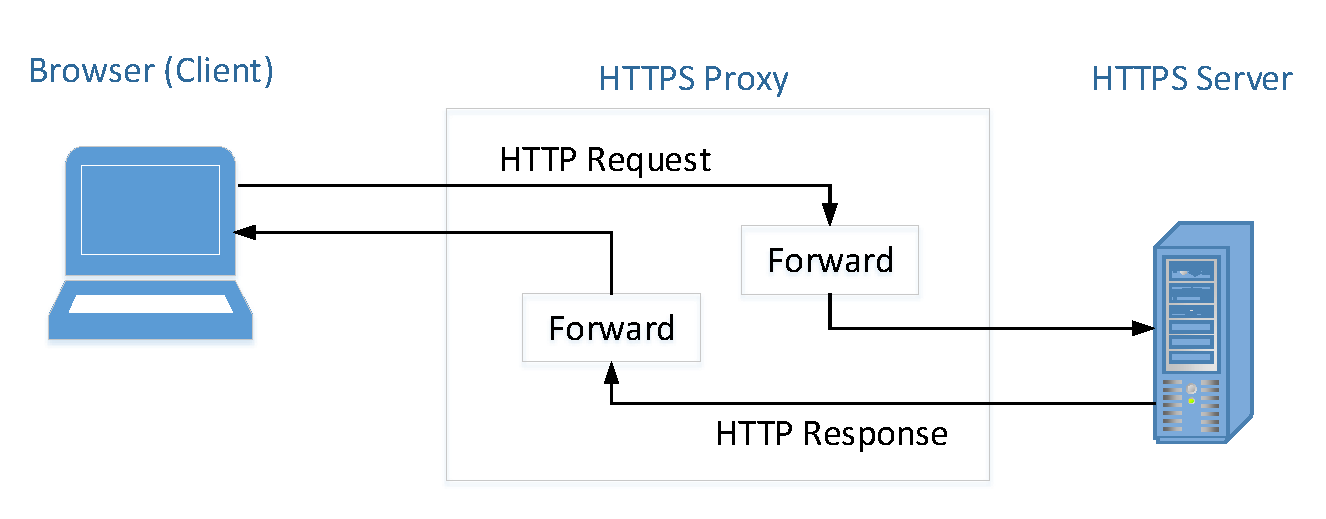
\includegraphics[width=0.8\textwidth]{\tlsFigs/httpsproxy.pdf}
\end{center}
\caption{How \texttt{mHTTPSproxy} works}
\label{tls:fig:proxy}
\end{figure}

The proxy is actually a combination of the TLS client and server programs.
To the browser, the TLS proxy is just a server program, which takes 
the HTTP requests from the browser (the client), and return HTTP
responses to it. The proxy does not generate any HTTP responses; instead,
it forwards the HTTP requests to the actual web server, and then 
get the HTTP responses from the web server. To the actual web server,
the TLS proxy is just a client program. After getting the response,
the proxy forwards the response to the browser, the real client. 
Therefore, by integrating the client and server programs implemented
in the previous two tasks, students should be able to get a basic 
proxy working. 


It should be noted that the purpose of this task is to use 
this simple proxy to understand 
how the Man-In-The-Middle attack works when the 
PKI infrastructure is compromised. It is not intended 
to implement a product-quality HTTPS proxy, because
making the proxy work for every web server is not an 
easy job, as many aspects of the HTTP protocol need to be 
considered. Since the focus of this lab is on TLS, 
students can choose two different servers, 
and demonstrate that their proxy works for those servers. 
Students who are interested in product-quality HTTPS proxy,
can find that from the Internet, such as the open-source
\texttt{mitmproxy}.  


\paragraph{Handling multiple HTTP requests.}
A browser may simultaneously send multiple HTTP requests to the server,
so after receiving an HTTP request from the browser, it is better to spawn a thread
to process that request, so the proxy program can handle multiple simultaneous
requests. The following code snippet shows how to create a thread to handle 
each TLS connection.

\begin{lstlisting}
import threading

while True:
    sock_for_browser, fromaddr = sock_listen.accept()
    ssock_for_browser = context_srv.wrap_socket(sock_for_browser, 
                                                server_side=True)
    x = threading.Thread(target=process_request, args=(ssock_for_browser,))
    x.start()
\end{lstlisting}


The thread will execute the code in the \texttt{process\_request} function,
which forwards the HTTP request from the browser to the server, and 
then forward the HTTP response from the server to the browser. A code skeleton
is provided in the following:


\begin{lstlisting}
def process_request(ssock_for_browser):
    hostname = 'www.example.com'

    # Make a connection to the real server
    sock_for_server  = socket.create_connection((hostname, 443))
    ssock_for_server = ... # [Code omitted]: Wrap the socket using TLS

    request = ssock_for_browser.recv(2048)

    if request:
        # Forward request to server
        ssock_for_server.sendall(request)      

        # Get response from server, and forward it to browser
        response = ssock_for_server.recv(2048)
        while response:
            ssock_for_browser.sendall(response) # Forward to browser
            response = ssock_for_server.recv(2048)

    ssock_for_browser.shutdown(socket.SHUT_RDWR)
    ssock_for_browser.close()
\end{lstlisting}


\paragraph{The client Setup.} 
For this task, since we will use a browser, we will 
use the hosting VM as the client/victim, instead of using 
the client container. 
In the real-world attack, when the victim tries to visit
a web server (say \url{www.example.com}), we will launch attacks to redirect
the victim to our proxy. This is usually done by DNS attacks, BGP attacks, or other 
redirection attacks. We will not actually do such attacks. We simply 
add the following entry to the \texttt{/etc/hosts} file on the host VM (\texttt{10.9.0.143} 
is the IP address of the mitm-proxy container in our setup). 

\begin{lstlisting}
10.9.0.143   www.example.com
\end{lstlisting}

By doing the above, we simulates the result of redirection attacks:
the victim's traffic to \url{www.example.com} 
will be redirected to the attacker's VM, where your \texttt{mHTTPSproxy} 
is waiting for HTTP requests. 
 

\paragraph{Task.} Students should implement the simple \texttt{mHTTPSproxy},
and run it on the proxy container. 
In this MITM attack, we assume that the attacker has compromised a trusted CA, and is 
able to use the CA's private key to generate fake (but valid) certificates for any
domain name. In this lab, the CA certificate generated in Task 2
is already trusted by the browser, and we assume this CA's private key
is compromised, so you/attacker can use it to forge certificate for any web server. 
Please demonstrate your MITM attack in the following scenarios:


\begin{itemize}

\item Launch the MITM attack against your own server. 

\item Launch the MITM attack on a real HTTPS website. You can pick 
a website. Find one that requires login, and then use your MITM proxy to 
steal the password. Many popular servers, such as facebook, have complicated 
login mechanisms, so feel free to find a server that has simple login mechanisms. 
Please remember to hide your password in your lab report if you 
are using a real password. 
\end{itemize}



\paragraph{Cleanup.} After finishing this task, 
please remember to remove the CA's certificate from your browser, and 
also remove any entry that you have added to \texttt{/etc/hosts} 
on your VM.



% *******************************************
% SECTION
% ******************************************* 
\section{Submission}

%%%%%%%%%%%%%%%%%%%%%%%%%%%%%%%%%%%%%%%%

You need to submit a detailed lab report, with screenshots,
to describe what you have done and what you have observed.
You also need to provide explanation
to the observations that are interesting or surprising.
Please also list the important code snippets followed by
explanation. Simply attaching code without any explanation will not
receive credits.

%%%%%%%%%%%%%%%%%%%%%%%%%%%%%%%%%%%%%%%%

\end{document}







